\chapter{DESIGN AND IMPLEMENTATION}
\label{chap:desainandimplementation}

% Ubah bagian-bagian berikut dengan isi dari desain dan implementasi

This chapter describes the design and implementation of the system that has been created.
As seen in Figure \ref{fig:block-diagram}, there are 2 main block diagrams. The left one is a block diagram for RECORD mode and the right one is for PLAY mode.
In RECORD mode, it starts with a human image and then does pose estimation to get human keypoints. After that, we convert the angle between 2 keypoints into a servo value so we can move the robot's servo to mimic human movement and save it for PLAY mode.
On the other hand, in PLAY mode, the input is 2: human image and humanoid robot image. Then, we perform pose estimation for both images. Before doing keypoint normalization, we have to choose 6 human keypoints based on humanoid robot keypoints. Lastly, we compare those keypoints and get the result.
\begin{figure}[ht]
  \centering
  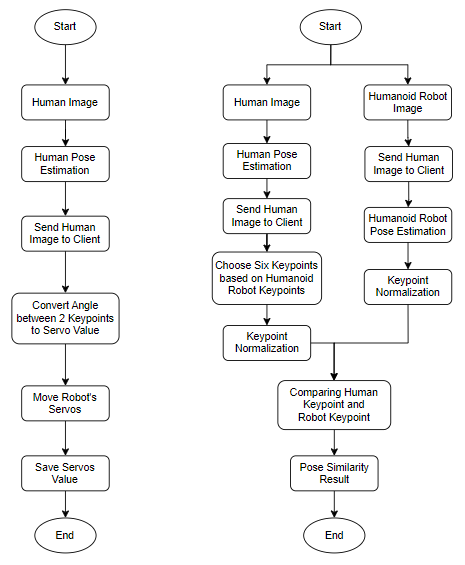
\includegraphics[scale=1.23]{gambar/diagram-block-revisi.png}
  \caption{Block Diagram of Workflow.}
  \label{fig:block-diagram}
\end{figure}
In the section that follows, each block is explained in further depth. Note that maybe there is a merge explanation if we use the same technique for different blocks. For instance, a block that sends a human image to the client and the block that send a robot image to the client will be merged to become just send an image to the client.


\section{Input Image}
\label{sec:input-image}

The input image that is fed into both models (human and humanoid robot) is 640x480 pixels with RGB channels. The device for getting the image is the Logitech C920 Webcam. We use OpenCV library to open the camera and capture the image.


\section{Human Pose Estimation}
\label{sec:human-pose-estimation}

Since there are already many pose estimation models for humans out there, we do not need to retrain them and just compare them to find the best model. In order to compare the models, we selected a paper for reference.
So evaluation metrics based on paper and real detection results will be shown in Chapter \ref{chap:resultsandiscussion} but for inference time, we will try in NUC i5. The models that we compare include OpenPose, MediaPipe, and YOLO-pose.
The input for these models is an RGB image and the output is the location of human keypoints.


\section{Send Image to Client}
\label{sec:send-image-to-client}

Our main program uses websites to interact with users because of its flexibility on any platform, the website view can be seen in Figure \ref{fig:websiteview}. So there is a Javascript client and a Python Server that communicate via \emph{socketio}.
The server will send human image to the client so we can adjust our position in the camera. This is done to enable the robot to capture the entire human pose.
\begin{figure}[ht]
  \centering
  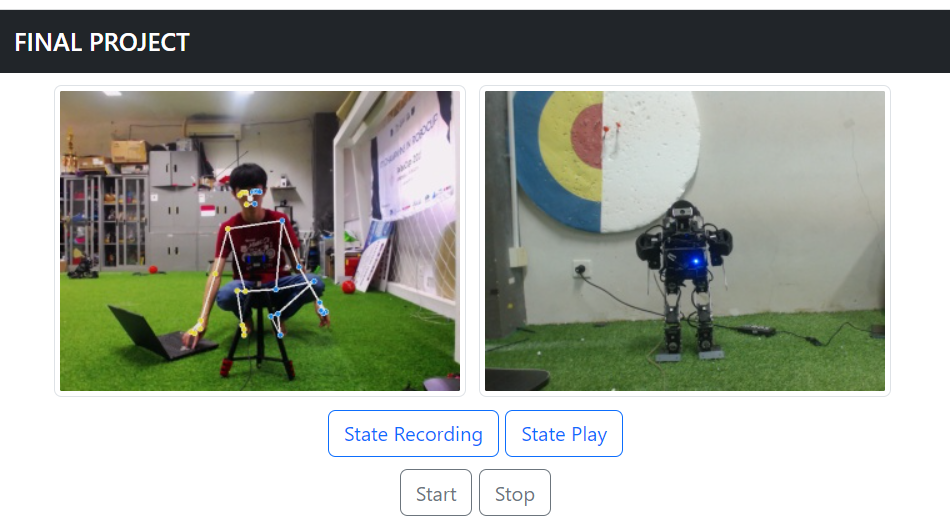
\includegraphics[scale=0.7]{gambar/web.png}
  \caption{Website View.}
  \label{fig:websiteview}
\end{figure}
The main program is divided into two modes, RECORD mode and PLAY mode. In RECORD mode, a human as a trainer gives a series of movements and will be followed by a humanoid robot, as well as robot saves these movements to use in PLAY mode later.
Meanwhile, in the PLAY mode, the robot acts as a trainer and performs a series of movements according to the movements previously stored in RECORD mode. Human will follow the robot's movement while the robot is also saving both human and robot images and comparing them later.

After getting human's keypoint, the server will visualize the detection result and send it as a buffer to the client.
On the client side, we use ReactJS library. There are four buttons: RECORD, PLAY, START, and STOP button. The RECORD and PLAY button indicates the modes in the main program, while the START and STOP button tell us when the mode is started or stopped.
There is a different color after we click on a button to indicate that we have pressed that button.
Apart from that, there are also two images that show human and robot image, actually in RECORD mode there is only one image (human image), while in PLAY mode there are 2 images (human and robot image). 
In our program, we define that client and server communicate through port 5555, where server can send image to client and client can send some data back to the server like current mode and time to start or stop the mode.
We use the \emph{useEffect} function to indicate if there is a change in a particular variable and do something like converting the image from the buffer to a string in order to display it on the HTML image tag.


\section{Convert Angle to Servo Value}
\label{sec:convert-angle-to-servo-value}

This section and Section \ref{sec:move-robot-servo} are triggered when the button RECORD and START is pressed on the website, so the client sends this information to the server and it does the calculation. 
To be able to move a robot's upper body like human movement, we need to obtain the angle between 2 keypoint using the \emph{arc tangent} function with the input \emph{\{x,y\}} keypoint coordinate.
Since we use MediaPipe Pose to detect human keypoints based on the result and discussion in Section \ref{sec:humanmodelcomparison}, the output is a normalized point, so we multiplied the x and y coordinates with the width and height image respectively to get the real pixel value.
Afterward, we subtract the second y keypoint value with the first y keypoint value and divided it by the second x keypoint value subtract with the first x keypoint value, and input the result to the \emph{arc tangent} function, as shown in Equation \ref{eq:arctan}.
\begin{equation}
  \label{eq:arctan}
  angle = \arctan \left(\frac{Y_2 - Y_1}{X_2 - X_1}\right)
\end{equation}

There are four angles we want to retrieve which are the angles from the shoulder to the elbow (right and left) and also the elbow to wrist (right and left) in order to robot can mimic upper body human movement.
If we look at MediaPipe Pose Landmark in Figure \ref{fig:mediapipe-landmark}, 6 keypoints that become our concern are 11, 12 for shoulders, 13, 14 for elbows, 15, and 16 for wrists. 
We get the right shoulder values by entering landmark 14 as the second argument and landmark 12 as the first argument of the \emph{arc tangent} function. This also applies to get the left shoulder angle value by entering landmarks 13 and 11 respectively. 
It is slightly different to obtain the elbow angles because we want its angle to be relative to the shoulder angle by subtracting its angle from the shoulder angle. We also apply limitations for each angle to keep the servo safe and not hit the robot body or other servo as seen in Table \ref{tb:robot-servos}.

\begin{longtable}{ccc}
  \caption{Robot Servos Limitations.}
  \label{tb:robot-servos}\\
  \hline
  \rowcolor[HTML]{C0C0C0}
  \textbf{Joint Angle} & \textbf{Motion} & \textbf{Range (deg)} \\
  \hline
  LShoulderPitch       & Left shoulder joint right and left    & -110 to 30  \\
  RShoulderPitch       & Right shoulder joint right and left   & -30 to 110 \\
  \rowcolor[HTML]{C0C0C0}
  \textbf{Joint Angle} & \textbf{Motion} & \textbf{Range (deg)} \\
  \hline
  LElbowRoll           & Left Elbow joint front and back       & -120 to 10  \\
  RElbowRoll           & Left Elbow joint front and back       & -10 to 120  \\
  \hline
\end{longtable}


\section{Move Robot's Servos}
\label{sec:move-robot-servo}

The program to move the robot's servos takes the same place as the program for the server. Our main program uses ROS2 with Python language. To be able to run the server and ROS2 program simultaneously, we need a separate thread, so the server program does not block the ROS2.
In the ROS2 framework, every package has its own functionality. On this occasion, we divide the task to move the robot's servo into 2 packages. The first one is named \emph{motion matching} where the server program and angle conversion to servo value happen, the other one is \emph{tachimawari},
a package that provides a DYNAMIXEL's joints management library for a ROS 2 project. This package name comes from a Japanese word that means motion. Every package has a node with the package's name like Figure \ref{fig:relation-node-record-mode}.
We can see this node relationship from rqt graph or ROS2 client interfaces, but we choose rqt graph because it is more visual.
\begin{figure}[ht]
  \centering
  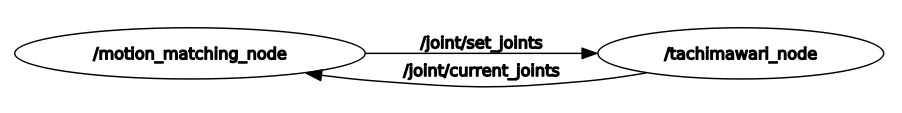
\includegraphics[scale=0.62]{gambar/rqt_without_akushon.png}
  \caption{Relationship Between Nodes in RECORD Mode.}
  \label{fig:relation-node-record-mode}
\end{figure}

Each node communicates with each other through a topic. There are 2 topics in RECORD mode, which are \verb|joint/set_joints| and \verb|joint/current_joints|. 
After getting desired servos angle from the previous section, we just need to publish it to \emph{tachimawari} node and it will move the servos. In the \emph{motion matching} node, there is a publisher that publishes servos angle to \verb|joint/set_joints| topic after the detection process and calculation is done, and also a subscriber in \emph{tachimawari} node that subscribes
to the same topic which collects the data that is published from the publisher. \verb|joint/set_joints| topic uses an interface like code snippet \ref{lst:set-joint-msg}, where there are \verb|control_type| variable with type integer and an array with Joint type, each joint consist of id and position like code snippet \ref{lst:joint-msg}.
\begin{lstlisting}[
  language={},
  caption={Joint msg.},
  label={lst:joint-msg}
]
uint8 id
float32 position
\end{lstlisting}

\begin{lstlisting}[
  language={},
  caption={SetJoints msg.},
  label={lst:set-joint-msg}
]
int8 control_type 4
Joint[] joints
\end{lstlisting}

In \verb|tachimawari_node| there is \verb|joint_node| that publishes the current joints every 8ms (it is used in the following section) and has a subscriber that listens to joints that we want to move. 
In order to move servos to the value that we want, we must enable the torque of all servos first. Then we make a command in array form that contains the servo's id and our desired value or target value (16 bytes) that split into 2 * 8 bytes.
For example, our target value is 512 (in binary is equal to \verb|00000010 00000000|), and the message that we send is 2 (\verb|00000010|) and 0 (\verb|00000000|). We can acquire that by performing bitwise AND and bitwise right shift. The bitwise AND operation is performed between the target value and \verb|0xFF|, which is represented as \verb|00000000 11111111| in binary.
Since \verb|0xFF| has 0 bits in the higher byte and 1 bits in the lower byte, the result of the operation is the lower byte of the target value. On the other hand, the bitwise right shift operator is used to shift the bits of the target servo 8 positions to the right. Shifting the bits to the right by 8 positions effectively discards the lower byte, leaving only the higher byte in the result.
It is the same when we receive the present position from the servo, the servo also sends the data in two bytes (lower and higher) and we need to combine the lower and higher bytes to reconstruct the 16-bit value representing the present position. This can be achieved by performing a left shift operation on the higher byte. Shifting it 8 bits to the left effectively moves it to the higher-order byte position.
After that, the bitwise OR operator combines the shifted higher byte with the lower byte. This operation merges the two bytes to form a 16-bit value representing the present position.


\section{Save Servos Value}
\label{sec:save-servo-value}

In the previous section, we discussed a little about the publisher in \emph{tachimawari} package that publishes the value of every current joint of the robot through a \verb|joint/current_joints| topic.
There is also a subscriber in \verb|motion_matching| node that is retrieved that data and a ROS2 timer that is triggered every 0.5 seconds to save the current joints in a JSON format like code snippet \ref{lst:json-save-joints} so our robot can move according to the movements exemplified by humans. 
The provided JSON format represents a structured data object that describes a specific action or movement sequence. There is "poses" array contains multiple pose objects, each representing a particular joint configuration during the action.
Each pose object includes a "joints" sub-object, which lists different joints and their corresponding values. For example, \verb|"left_ankle_pitch"| has a value of 25, \verb|"left_ankle_roll"| is set to 0, and so on. These values represent the positions or angles of the respective joints.
Each pose object also has a "name" field to identify the pose. The "pause" field specifies the duration of the pause between this pose and the next one, while the "speed" field indicates how fast this pose will be executed.
Lastly, the \verb|"start_delay"| field denotes any delay before the action begins, and the \verb|"stop_delay"| field signifies the delay after the action finishes before the robot stops. In total, there are 20 servos in our robot, so in the actual JSON file each "joint" sub-object has 20 items with their respective joint names.

\begin{lstlisting}[
  language={},
  caption={JSON Format to Save Joints Value.},
  label={lst:json-save-joints}
]

  "poses": [
    {
      "joints": {
        "left_ankle_pitch": 25,
        "left_ankle_roll": 0,
        ...
      },
      "name": "pose name",
      "pause": 0,
      "speed": 0.003
    },
  ],
  "start_delay": 0,
  "stop_delay": 0

\end{lstlisting}


\section{Humanoid Robot Pose Estimation}
\label{sec:humanoid-robot-pose-estimation}

This explanation is intended for the right block diagram from Figure \ref{fig:block-diagram} or we can also say as the RECORD mode. The difference between the PLAY and RECORD modes lies in the number of cameras used.
So there will be two cameras, one camera to record human movement (located on the robot's head) and the other to record robot movement (located from the human side facing the robot), the distance between them approximately 1 - 1.5 meters, as shown in Figure \ref{fig:pose-comparison-side}.
In PLAY mode, the server side sends two images so that we can know and adjust the position of humans and robots in the camera. Due to the large network delay when sending two 320x240 pixel images, when the START button is pressed,
the server does not send the image to client again, the robot plays a series of moves stored in the previous JSON file by communicating via another ROS2 packages, while saving both images. After that, when the STOP button is pressed, the server starts to compare poses between them.
\begin{figure}[ht]
  \centering
  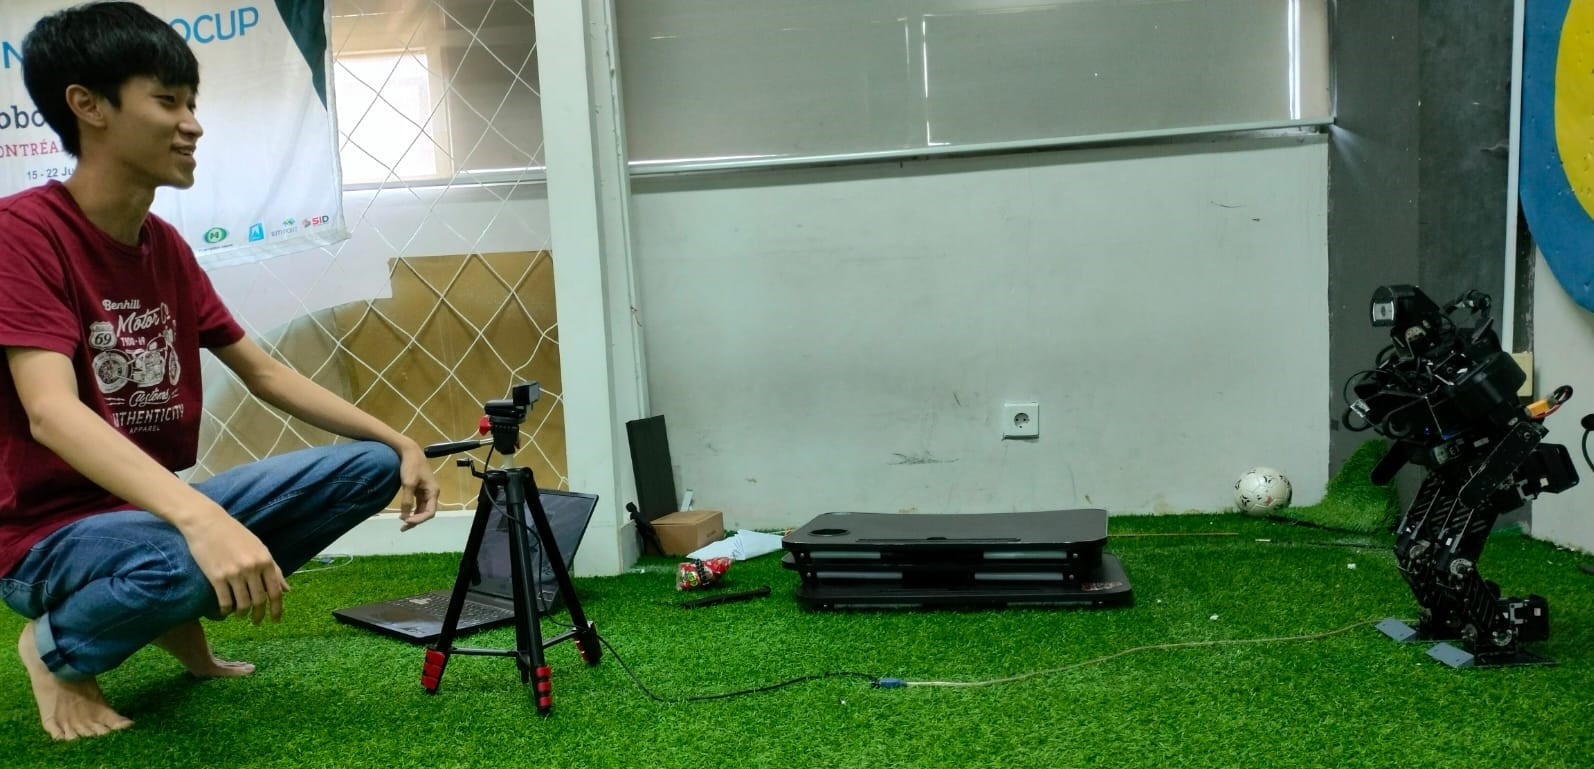
\includegraphics[scale=0.3]{gambar/pose-comparison.jpeg}
  \caption{Pose Comparison from Side.}
  \label{fig:pose-comparison-side}
\end{figure}

This section immediately begins with the estimation pose for humanoid robot because the explanation regarding the previous block has been explained in the previous section.
Since there are not many pose estimation models for humanoid robots out there yet, we need to retrain them or use transfer learning from the model that supposes to estimate human pose.
Therefore, the first step is making a new humanoid robot pose dataset.

\subsection{Make New Dataset}
\label{subsec:make-new-dataset}

This new dataset is a merge of NimbRo's Humanoid Robot Pose dataset and Ichiro's dataset. NimbRo's dataset contains both single and multiple robots to
simulate RoboCup's real conditions. They also gathered from RoboCup Humanoid League YouTube videos, their own internal videos, and ROS bags. 
Overall, their dataset has over 1.5k images that come from 23 videos with around 2.3k robot instances. These images include teen and adult-sized robots and contain more than ten different robot types \parencite{amini2021}.
However, the robots in Ichiro's dataset are only kid-sized and come in single or maximum two-robot configurations. The images in our dataset come from videos that are taken in our lab. 
Then we split up those videos into multiple images and we pick not blurred videos.
Before merging, we need to fix NimbRo's dataset format first. This is because after we visualized some of their data, we found that the bounding boxes in \emph{annotations} part were misplaced (the width and height were swapped).
After we refine their dataset format and merge them with our dataset, the newly created dataset has approximately 2.1k images.
About 20 percent of the dataset was used for scoring and validating.

When it comes to annotation tools, there are a lot of choices out there including offline and online tools. We have tried some of them like Dataloop, V7labs, or Supervisely which is recommended by NimbRo.
However, when we tried to export the dataset into COCO format, it failed (e.g. can not import it or it can be imported but the JSON result in the annotation section is none). So, we decided to use a coco-annotator,
a web-based image annotation tool designed for versatility and efficiently labeling images to create training data. Regarding the number of keypoints in each robot, we followed NimbRo's dataset.
There are six keypoints including head, trunk, hands, and feet. We stick to that idea because we want to try the model's performance and inference time with fewer keypoints first and if we are confident enough, we will increase the number of keypoints later.

\subsection{Training Pose Estimation Model for Humanoid Robot}
\label{subsec:training-robot}

All of the training processes in this study were primarily conducted on a DGX-A100 server computer and written in the Python programing language. The specific configuration explains in Table \ref{tb:dgxa100}.
From this base specification, we are allocated a Jupiter notebook container with
python and many libraries preinstalled with following allocated resources explained in Table \ref{tb:allocatedcontainer}.
\begin{longtable}{|c|c|}
  \caption{DGX-A100 Specification.}
  \label{tb:dgxa100}\\
  \hline
  CPU     & Dual AMD Rome 7742, 128 cores total @ 2.25 GHz \\
  \hline
  GPU     & 8 x NVIDIA A100 80 GB Tensor Core GPUs  \\
  \hline
  RAM     & 2 TB \\
  \hline
  Storage & 30 TB (8 x 3.84 TB) U.2 NVMe drives \\
  \hline
\end{longtable}

\begin{longtable}{|c|c|}
  \caption{Allocated container specification.}
  \label{tb:allocatedcontainer}\\
  \hline
  GPU     & 1/8 NVIDIA A100 GPU \\
  \hline
  GPU RAM & 10 GB  \\
  \hline
  CPU RAM & 8 GB \\
  \hline
  Storage & 100 GB  \\
  \hline
\end{longtable}

\subsubsection{NimbRo's Model}
\label{subsubsec:training-nimbro-model}

The hyperparameters that are used to train NimbRo's model followed the description in their paper.
This model is trained using the AdamW optimizer with a learning rate of 10\textsuperscript{-4},
batch size 16, and weight decay of 10\textsuperscript{-4} for the total 200 epochs.
Note that the encoder is initialized by pre-trained ResNet weights on ImageNet.
We also use data augmentation that includes random scaling and random translation during training \parencite{amini2021}.
We do not use random horizontal flip and random rotation like NimbRo did because in our case it will make the training result worse.

The main program for training is already made by them named \emph{main.py} using PyTorch framework, we just need to run it on Jupyter Notebook file or Terminal and adjust the arguments for our needs.
In their script, there is an argument name \verb|config| which it is referred to a file where we store all the hyperparameters, number of epochs, dataset name for training and testing, and many others. 
Another argument tells us about a directory path where we save training results and the dataset takes place.
\lstinputlisting[
  language={},
  caption={Example YAML file config for NimbRo's Training.},
  label={lst:confignimbro}
]{files/train_nimbro.yaml}
File \ref{lst:confignimbro} is an example of YAML configuration file for NimbRo Training. This is not a complete version, but we included parts that were changed frequently during the training process.
The "SEED" is set to 42, ensuring reproducibility of random processes. The "DEVICE" is specified as "cuda", indicating the utilization of a GPU for computation.
\verb|"BATCH_SIZE"| is set to 16, meaning that 16 data samples will be processed together in each training iteration. If we make \emph{batch size} value larger, it requires more memory to store the input data, intermediate activations, and gradients during training.
If the available memory is limited, increasing the batch size beyond the memory capacity may lead to out-of-memory errors or cause the training process to slow down.
However, larger batch sizes can speed up the training process as more samples are processed in parallel. It also effect the generalization capability of the model.
Smaller batch sizes tend to provide more stochasticity during training, which can act as a form of regularization and help prevent overfitting. In contrast, larger batch sizes may result in a smoother optimization process, potentially leading to faster convergence but with a slightly increased risk of overfitting.
The \verb|"NUM_WORKERS"| is set to 2, indicating that two worker processes will be used to load and preprocess the data.

The training process will run for 200 epochs as specified by \verb|"NUM_EPOCHS"|. When training for more epochs, the model undergoes more iterations and updates, allowing it to refine its learned representations and adjust its parameters based on the training data.
This can lead to improved model performance as the model converges towards an optimal solution and achieves higher accuracy on both the training and validation data. However, it is important to be cautious of the risk of overfitting. Overfitting occurs when the model becomes too specialized to the training data and fails to generalize well to unseen data.
Increasing the number of epochs without proper regularization techniques can increase this risk. The model may start to memorize the training data instead of learning generalizable patterns, resulting in poor performance on new data. Additionally, training for a greater number of epochs requires more time.
The \verb|"PRINT_FREQ"| is set to 100, meaning that training progress and relevant information will be printed or displayed every 100 iterations.

The "DATASET" section contains settings related to the dataset used for training.
The \verb|"DATASET.TRAIN"| specifies the name or identifier of the training dataset folder, and \verb|"DATASET| \verb|.TEST"| indicates the name of the validation dataset folder. The \verb|"NUM_KEYPOINTS"| is set to 6, denoting the number of keypoints or landmarks in the dataset, while \verb|"NUM_LIMBS"| is set to 5, representing the number of limbs or connections between keypoints.
The \verb|"MAX_NUM_| \verb|DETECTIONS"| is set to 10, indicating the maximum number of robots in the dataset. The "SIGMA" parameter is set to 2.0, which is used in generating heatmaps. For augmentation, The "FLIP" is set to 0.0, meaning there will be no horizontal flipping of the input data. The "TRANSLATE" is set to 0.4, allowing the data to be translated by up to 40\% of its size.
The "SCALE" parameter represents a range of scaling applied to the input data, with a minimum scale of 0.5 and a maximum scale of 1.5. The "ROTATION" is set to 0, indicating no rotation will be applied to the input data. Additionally, the \verb|"INPUT_SIZE"| is set to [384, 384], representing the desired input size of the model, while the \verb|"OUTPUT_SIZE"| is set to [192, 192], indicating the desired output size.

\subsubsection{YOLO-pose}
\label{subsubsec:training-yolo-pose}

Before we jumped into training process, we must change format of our newly dataset from COCO to YOLO. Differ from COCO format, YOLO format gives keypoint confidence or visibility flag 2 for either visible or occluded keypoint
and if it is outside the field of view, the value is set to zero. However, COCO format defines visibility flag as v=0: not labeled, v=1: labeled but not visible, and v=2: labeled and visible. So, we change the definition of
v=1 and v=2 become just v=2 in YOLO format and keep v=0. As seen in Pseudocode \ref{lst:change-keypoint-format}, where we make a function called \verb|change_keypoint_format| which has 2 input arguments and return new keypoints with YOLO format. 
Beside keypoint format differences, bounding-box format between them is also different. COCO defines a bounding-box as follow: x (top left), y (top left), width, and height. On the other hand,
bounding-box format in YOLO is: x (center), y (center), width, and height also all of them need to be normalized. Thus, we need to add 1/2 width to x, 1/2 height to y like in Pseudocode \ref{lst:change-bbox-format}, and normalize them by multiplying new x and y with 1/width and 1/height respectively. 

\lstinputlisting[
  language={},
  caption={Change Keypoint Format From COCO to YOLO.},
  label={lst:change-keypoint-format}
]{program/change-keypoint.txt}

\lstinputlisting[
  language={},
  caption={Change Bounding Box Format From COCO to YOLO.},
  label={lst:change-bbox-format}
]{program/bbox-norm.txt}

The hyperparameters to train YOLO-pose followed the description in their GitHub named \emph{hyp.pose.yaml}.
We use SGD optimizer with a cosine scheduler. The base learning rate is set to 10\textsuperscript{-2}, batch size 16,
and weight decay of 5\textsuperscript{-4} for total 150 epochs. There are also data augmentation like random scale ([0.5, 1.5]),
random translation [-10, 10], mosaic augmentation with probability 1, and various color augmentations.
It is the same with previous section, the main program for training has been provided using PyTorch framework too, but the program is intended for humans with 17 keypoints.
If we run it directly with our dataset with 6 keypoints, an error will be raised. Therefore, a little bit of code needs to be changed to make the training process can be run.

\subsubsection{Keypoint RCNN}
\label{subsubsec:training-rcnn}

The Keypoint RCNN training is done on Jupyter Notebook directly using the PyTorch framework as well.
Before starting the training process, we also need to convert the dataset format first.
Actually, this format is almost the same as the YOLO format (each image has its own label), but the difference lies in the bounding box.
Where the format of the bounding-box is the top left point and the bottom right point. We can obtain bottom right point by adding bounding box width to x coordinate and its height to y coordinate.

The training process starts with loading our dataset and specifying the augmentation technique we are using. We use \emph{albumentations} library from Python for augmenting our dataset.
At first, we apply random brightness, contrast, and rotation. Nevertheless, the model seems to become underfitting, so we try just random brightness and contrast. Fortunately, the result seems pretty good after that.
Before we declare RCNN model using torchvision library, we need anchors that will be an input argument. 
By default, the \emph{AnchorGenerator} class in PyTorch has 3 different sizes (128, 256, 512) and 3 different aspect ratios (0.5, 1.0, 2.0).
We have extended those parameters, \verb|sizes| to (32, 64, 128, 256, 512) which means that anchor boxes with different base sizes will be generated. These base sizes represent the approximate dimensions (in pixels) of the objects that the algorithm will try to detect.
The anchor generator will create anchors with these base sizes at different positions in the image.
The \verb|aspect_ratios| specifies the aspect ratios of the anchor boxes. Aspect ratio refers to the ratio of the width to the height of the anchor box.
The \verb|aspect_ratios| argument is set to (0.25, 0.5, 0.75, 1.0, 2.0, 3.0, 4.0), which means anchor boxes with these aspect ratios will be generated. By combining different base sizes and aspect ratios, the anchor generator can produce a diverse set of anchor boxes,
which are used as reference bounding boxes during the object detection process. These anchor boxes are later compared to the ground truth bounding boxes of objects in the training data to determine the location of objects.
Note that, \verb|num classes| argument is set to two because the first class is background and object is the second class.
In this training, we use SGD optimizer with learning rate 10\textsuperscript{-3}, batch size 3, and weight decay of 5\textsuperscript{-4} for 50 epochs.

\subsection{Finding the Best Model for Humanoid Robot Pose Estimation}
\label{subsec:finding-best-model-humanoid-robot}

After retraining 3 models on Section \ref{subsec:training-robot}, we try to find the best one for our case. We compare them based on \emph{mAP} (mean Average Precision), \emph{mAR} (mean Average Recall),
real detection result, and inference time on devices with limited computing capabilities (e.g. NUC i5).
The comparison table of \emph{mAP}, \emph{mAR}, and real detection result of those models are in Chapter \ref{chap:resultsandiscussion}. In this section we just talk about the time inference.
To know the time that it takes for the model to do the detection, we just need to subtract the time before and after the model does keypoint detection like Pseudocode \ref{lst:time-difference}.
In this pseudocode, the \verb|get_current_time()| function is used as a placeholder to represent the retrieval of the current time. The keypoint detection process is performed in the indicated section.
The \verb|elapsed_time| variable is calculated by subtracting the starting time from the current time. Finally, the elapsed time is printed with an appropriate message.

\lstinputlisting[
  language=Python,
  caption={Time difference Pseudocode.},
  label={lst:time-difference}
]{program/time-difference.txt}

We also attempt converting our models from PyTorch Model to OpenVINO in order to speed up the time inference. Before that, we convert it to ONNX first like Figure \ref{fig:pytorch-to-openvino}.
At first, we must ensure that the model is in inference mode by calling \emph{eval} function in Python code.
Next, we create that dummy input variable. The call to \emph{torch.onnx.export} function runs the model once to trace its execution and then exports the traced model to the specified file.
The resulting onnx file contains a binary protocol buffer which contains both the network structure and parameters of the model exported.
After that, we use Model Optimizer to convert the ONNX model to OpenVINO IR with FP16 precision. To install Model Optimizer in Python is pretty simple, just run
\emph{pip install openvino-dev} in Terminal and to verify the package is properly installed, we run the command \emph{mo -h}. We will see the help message for Model Optimizer if installation finished successfully.
After running that command, there is a directory that contains three files with \emph{bin}, \emph{mapping}, and \emph{xml} extension.
If we want to run OpenVINO IR Model in OpenVINO Runtime, we must make sure that the path for model must contain three files earlier.

\begin{figure}[ht]
  \centering
  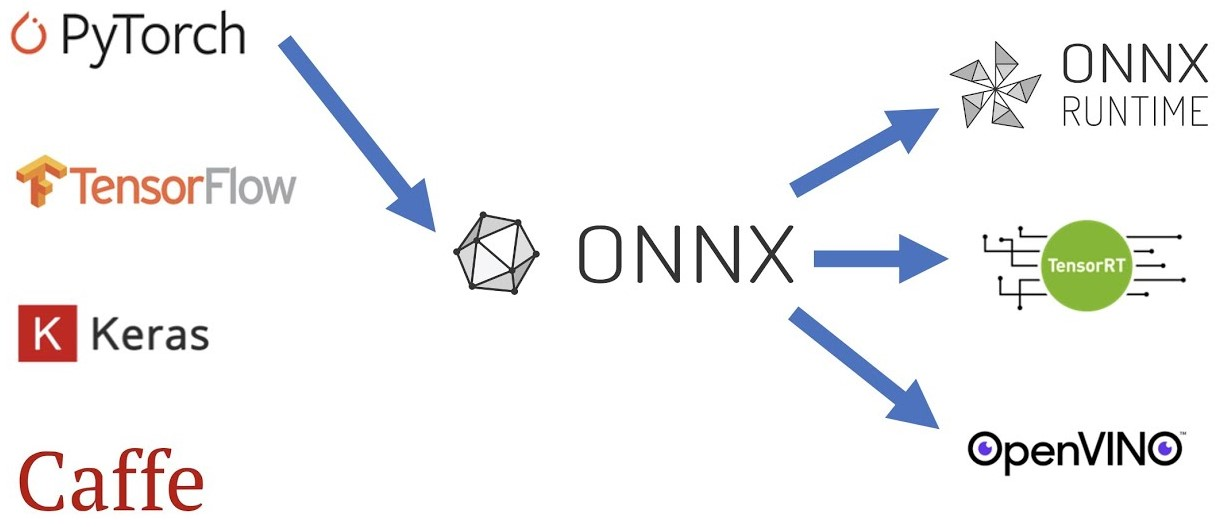
\includegraphics[scale=0.4]{gambar/pytorch-onnx-openvino.jpg}
  \caption{Flow of converting PyTorch Model to OpenVINO.}
  \label{fig:pytorch-to-openvino}
\end{figure}


\section{Choose Six Keypoints based on Humanoid Robot Keypoints}
\label{sec:choose-keypoints}

The difference in numbers between human keypoints and robot keypoints makes us have to choose certain human's keypoints in order to make a comparison between them.
Based on the results after testing, we chose Mediapipe for human and Keypoint RCNN for robot. Mediapipe provides 33 landmark keypoints for human and Keypoint RCNN only provides 6 keypoints.
Therefore, we need to choose 6 human keypoint as shown in Pseudocode \ref{lst:choose-human-keypoints}.
Note that, the name of the keypoints in the code corresponds to the name of the keypoints in the robot. First, we get all 33 keypoints. Then calculate the keypoint we want, such as the head keypoint which is located between the right and left eye.
To obtain the eye landmarks, we can index \verb|landmark| variable according to Figure \ref{fig:mediapipe-landmark}, where the left eye is index 2 and the right eye is index 5. This also applies to other landmarks.
The keypoint for the hands and feet is simply to select the wrists and ankles, where landmark[15] and landmark[16] are wrists, landmark[27] and landmark[28] are ankles.
Lastly, the trunk keypoint is located between the shoulder and hip keypoint. The x coordinate is located in the middle of the hip. The y-coordinate, on the other hand, is located on 1/4 distance between the hip and the shoulder from below.
First, we determine the midpoint between the shoulder and hip by individually calculating the coordinates of the right and left y axes, like Pseudocode \ref{lst:choose-human-keypoints} lines 19 and 21. In order to obtain 1/4 of the distance between the hip and the shoulder from below, we then compute the midpoint between the previous computation and the hip point as shown in lines 20, 22, and 24.
After all of the computation, we arrange all keypoints in a single array.

\lstinputlisting[
  language={},
  caption={Choose human keypoints.},
  label={lst:choose-human-keypoints}
]{program/choose-human-keypoints.txt}


\section{Keypoint Normalization}
\label{sec:keypoint-normalization}

When we think about the problem, we see that there are many uncertainties to be addressed. For example, human and humanoid robot can differ in height, body shape, and location within an image: one subject (human or robot) may have been nearby the camera,
while another may have been in the distance. In order to get an accurate outcome, each of these issues must be resolved.
After choosing the keypoints, the model output for both human and robot is the coordinates of 6 keypoints. This information can be used to create a new keypoint coordinates starting from (0,0) in the image. This solves the problem of the subject appearing in different parts of the picture.

\lstinputlisting[
  language={},
  caption={Get New Keypoints.},
  label={lst:new-keypoints}
  ]{program/bbox.txt}

In Pseudocode \ref{lst:new-keypoints}, the code is structured into two functions: \verb|get_min_point| and \verb|get_| \verb|new_coords|. The \verb|get_min_point| function takes an array of keypoints coordinates as input with shape (6,2)
and iterates through each item in the array. It keeps track of the minimum x and y values encountered during the iteration and returns an array containing the minimum x and y coordinates.
The \verb|get_new_coords| function takes the keypoint coordinates array and \verb|min_point| (minimum x and y coordinates) from the previous calculation as input. It iterates through each item and subtracts the corresponding minimum x and y values from each coordinate. The updated coords array is returned.

We further normalized the resulting keypoints coordinates by performing L2 normalization in order to transform it into a unit vector as shown in Figure \ref{fig:transforming-into-unit-vector}.
This means we are ignoring the size of the picture, but keeping in account the direction of the vector, created by the pose inside of that image.
To calculate the L2 normalization for an individual point is to take the square root of the sum of the squares of its coordinates. This calculation resulting the magnitude or length of the vector formed by the coordinates of the point.
Next step is dividing each coordinate by the length of the vector. This step ensures that the resulting normalized point lies on the unit circle. This normalization process scales the coordinates proportionally while preserving the direction of the vector. Moreover, it will optimize using NumPy library so it can compute multiple points simultaneously.

\begin{figure}[ht]
  \centering
  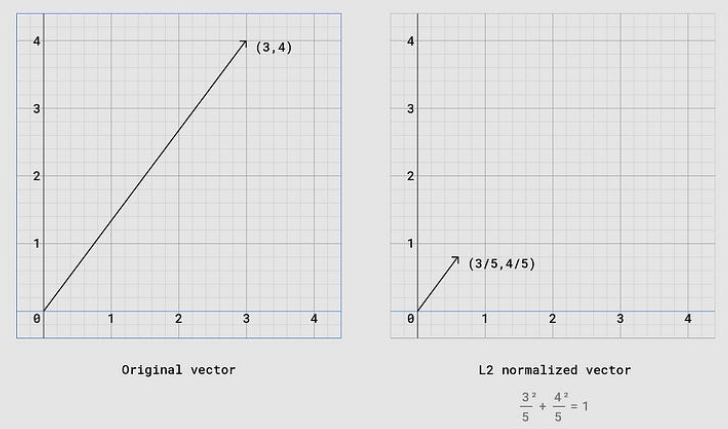
\includegraphics[scale=0.8]{gambar/transform-to-unit-vector.png}
  \caption{Transforming into Unit Vector.}
  \label{fig:transforming-into-unit-vector}
\end{figure}


\section{Comparing Human Keypoints and Robot Keypoints}
\label{sec:comparing-keypoints}

Now that we have standardized the pose vectors, it is time to choose a similarity measure. We chose cosine similarity for this particular instance, mainly because we are working with vectors and performing a few calculations detailed below to arrive at a Euclidean distance that can be interpreted as a cosine distance.
The cosine similarity ranges from -1 to 1, with 1 indicating identical poses or vectors are in the same direction, 0 indicating no similarity or vectors are nearly orthogonal, and -1 indicating completely opposite poses or opposite direction. The cosine distance, on the other hand, is a dissimilarity measure that ranges from 0 to 2.
Using Equation \ref{eq:euclideandistance} scales the values to the range of 0 to 2, making it easier to interpret the results. A larger value implies a greater dissimilarity between poses. In that equation, Fxy and Gxy are two pose vectors to be compared after L2 normalization. Moreover, Fxy and Gxy contain only x and y positions for each of the 6 keypoints, it does not include confidence scores.

\begin{equation}
  \label{eq:cosinesimilarity}
  cosineSimilarity(x,y) = \frac{x \cdot y}{|x||y|}
\end{equation}

\begin{equation}
  \label{eq:euclideandistance}
  D(F_{xy}, G_{xy}) = \sqrt{2 * (1 - cosineSimilarity(F_{xy}, G_{xy}))}
\end{equation}


\section{Pose Similarity Result}
\label{sec:pose-similarity-result}

The result of pose similarity is in percentages with a range of 0 to 100. A higher score indicates a more similar position between the human and robot, and vice versa.
In order to get it, we multiply the cosine distance result from Section \ref{sec:comparing-keypoints} by 100 and subtract the result from 100.
After getting each result of pose similarity, we take a mean and display it in the left top video. This video will be generated after detecting and comparing all poses.